\documentclass[final,hyperref={pdfpagelabels=false}]{beamer}
\mode<presentation>
  {
  %  \usetheme{Berlin}
  \usetheme{Dreuw}
  }
  \usepackage{times}
  \usepackage{amsmath,amsthm, amssymb, latexsym}
  \boldmath
  \usepackage[english]{babel}
  %\usepackage[latin1]{inputenc}
  \usepackage[orientation=portrait,size=a0,scale=1.4,debug]{beamerposter}

  \usepackage{fancybox}
  \usepackage{CJKutf8}


  %%%%%%%%%%%%%%%%%%%%%%%%%%%%%%%%%%%%%%%%%%%%%%%%%%%%%%%%%%%%%%%%%%%%%%%%%%%%%%%%%5
  \graphicspath{{figures/}}
  \title[]{Nders at the NTCIR-13 Short Text Conversation 2 Task}
  \author[]{Han Ni, Liansheng Lin, Ge Xu}
  \institute[ND]{NetDragon WebSoft Inc.}
  %\date{Jul. 31th, 2007}


  %%%%%%%%%%%%%%%%%%%%%%%%%%%%%%%%%%%%%%%%%%%%%%%%%%%%%%%%%%%%%%%%%%%%%%%%%%%%%%%%%5
  \begin{document}
  \begin{frame}{} 
    %\vfill
    
      \begin{columns}[t]
        \begin{column}{.49\linewidth}
          \begin{block}{\large Introduction}
            This poster describes our retrieval-based approaches at NTCIR-13 short text conversation 2 
            (STC-2) task (Chinese). \\
            For a new post, our system firstly retrieves similar posts 
            in the repository to get their corresponding comments, and then finds the 
            related comments directly from the repository. \\ 
            Moreover, we devise two new methods: \\
            1) LSTM-Sen2Vec model to get the vector of sentence. \\
            2) Pattern-IDF to rank the candidates from above. \\
            Our best run achieves 0.4780 for mean nG@1, 
            0.5497 for mean P+, and 0.5882 for mean nERR@10, and respectively rankes 4th, 
            5th, 5th among 22 teams.
          \end{block}
        \end{column}
        \begin{column}{.49\linewidth}
          \begin{block}{\large Example from Our Results}
          \centering
          \vskip0.5ex

          \begin{table}
          \centering
          %\caption{Short Text Conversation}
          \setlength\tabcolsep{1cm}
          \begin{tabular}{ll}
          \hline
           Post      & {\scriptsize \begin{CJK}{UTF8}{gbsn}好喜欢这种手绘的画啊,小柚子加油\end{CJK}} \\ 
                     & {\scriptsize Really like this hand-painted painting, xiaoyouzi, come on! } \\
          \hline
           Comment 1 & {\scriptsize \begin{CJK}{UTF8}{gbsn}喜欢这种手绘我也要画\end{CJK} }\\ %\hline
                     & {\scriptsize Like this hand-painted painting, I also want to draw it.} \\
          \hline
           Comment 2 & {\scriptsize \begin{CJK}{UTF8}{gbsn}我想问你的画是手绘还是电脑画的啊\end{CJK} } \\ %\hline
                     & {\scriptsize I want to ask whether your paintings are hand-painted or computer painted.} \\
          \hline
           Comment 3 & {\scriptsize \begin{CJK}{UTF8}{gbsn}这是用电脑画的还是手绘的?\end{CJK} } \\ %\hline
                     & {\scriptsize Was this drawn by computer or hand-painted ?} \\
          \hline
           Comment 4 & {\scriptsize \begin{CJK}{UTF8}{gbsn}很有爱的画。是用手绘板画的么?\end{CJK} }\\ %\hline
                     & {\scriptsize It's a lovely painting. Was it painted with a hand-painted board?} \\
          \hline
  
          \end{tabular}
          \end{table}
        \vskip0.3ex
          \end{block}
        \end{column}
      \end{columns}  
    %\vfill
    %\vfill
    \vskip1ex


    \begin{block}{\large Our System}
      \begin{columns}[t]
        \begin{column}{.48\linewidth}
            \centering
            \begin{block}{\Large Preprocessing}
              \begin{itemize}
                \item {\normalsize Convert traditional Chinese into simplified Chinese}
                \item {\normalsize Convert full-width characters into half-width ones}
                \item {\normalsize Replace all the number, datetime, url with token \_NUM, \_TIME, \_URL respectively}
                \item {\normalsize Word Segmentation}
                \item {\normalsize Filter meaningless words and symbols}
              \end{itemize}
            \end{block}
            
            \vskip1.5ex

            \begin{block}{\Large Candidates Generation} 
              \begin{itemize}
                \item {\normalsize Train Word2Vec, LSA, LDA and LSTM-Sen2Vec models on the repository and convert sentence into vector}
                \item {\normalsize Use cosine similarity to calculate similarity between two vectors}
                \item {\normalsize Retrieve similar posts with Word2Vec, LSA/LDA and LSTM-Sen2Vec models}
                \item {\normalsize Get corresponding comments from the similar posts as part of comment candidates}
                \item {\normalsize Retrieve appropriate comments directly from all comments with Word2Vec and LSA/LDA models}
                \item {\normalsize Combine two candidates as the final comment candidates}
              \end{itemize}
            \end{block}

            \vskip1.5ex

            \begin{block}{\Large Ranking}
              \begin{itemize}
                \item {\normalsize Use graph-based algorithm TextRank to rank the candidates}
                \item {\normalsize Use Pattern-IDF to rank the candidates}
                \item {\normalsize Use Pattern-IDF and TextRank to rank the candidates}
              \end{itemize}
            \end{block}

          %\end{itemize}
    
        \end{column}
        \begin{column}{.48\linewidth}
          \centering
          %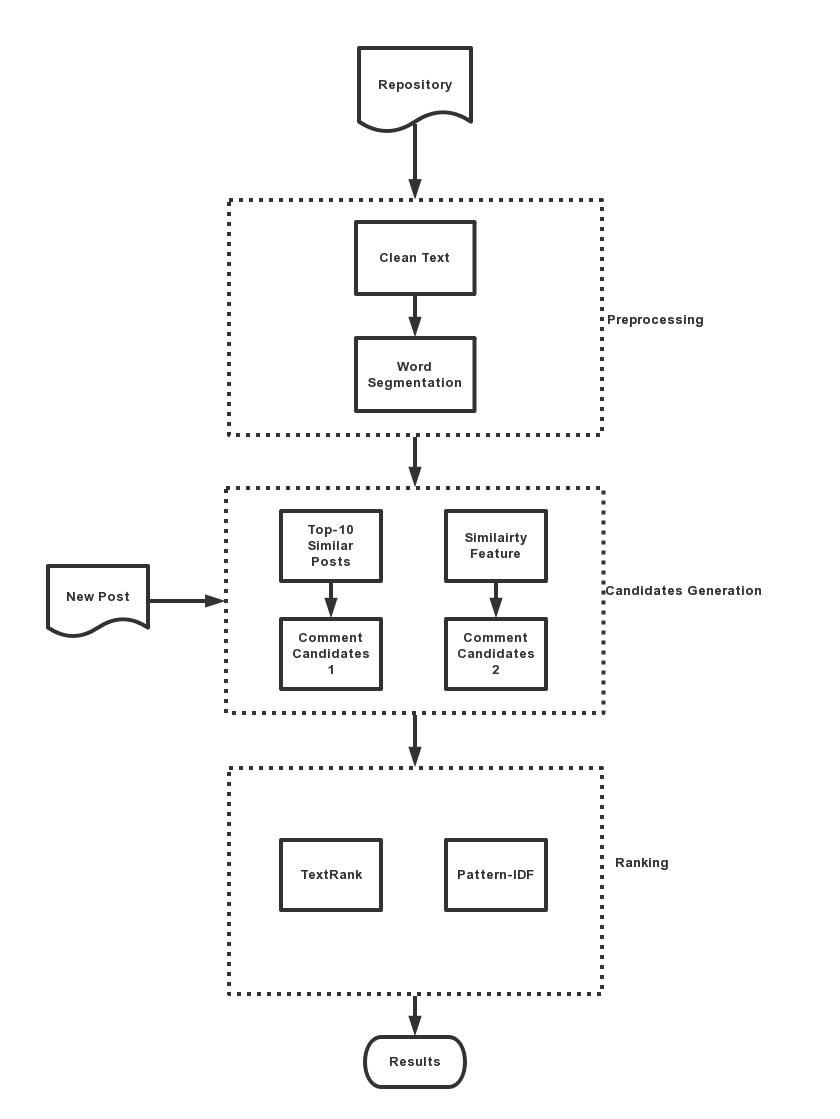
\includegraphics[width=40cm, height=60cm]{stc-flow.png}
          \begin{figure}
            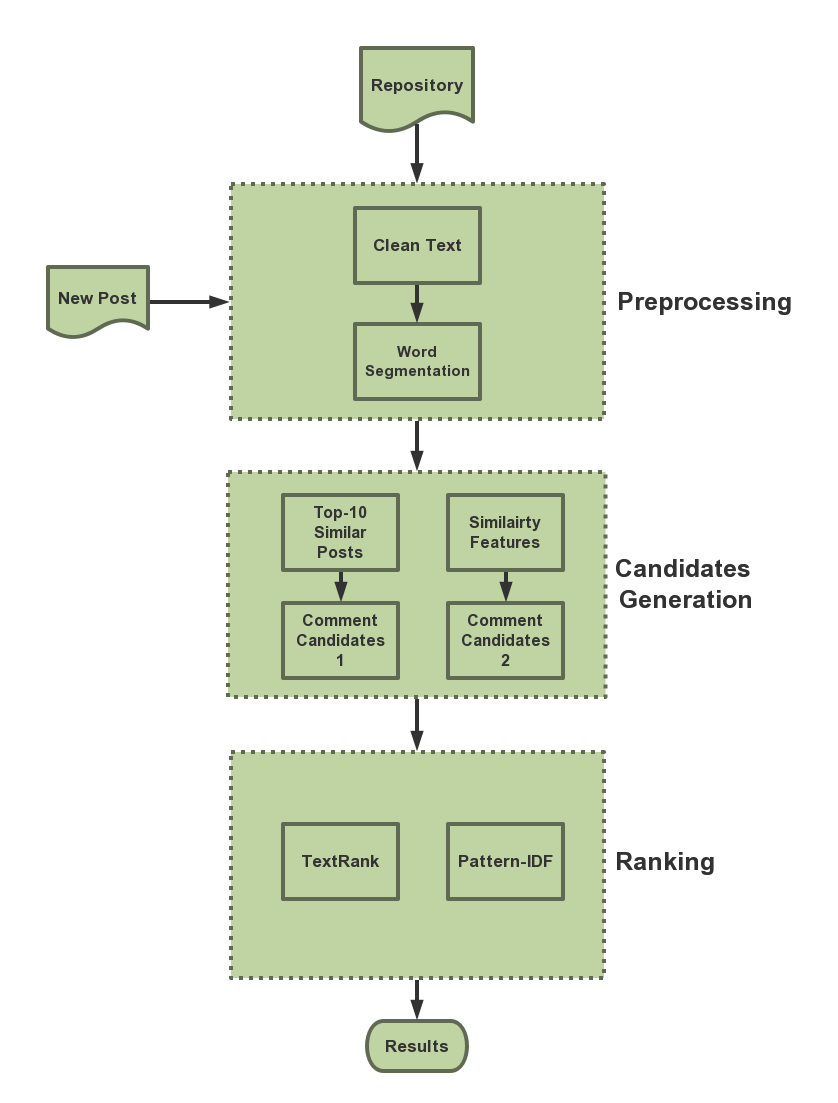
\includegraphics[width=36cm, height=47.38cm]{stc-flow4.png}
            \caption{System Architecture}
          \end{figure}
        \end{column}
      \end{columns}
      
    \end{block}
    %\vfill
    \begin{columns}[t]
      \begin{column}{.49\linewidth}
        \begin{block}{Experimental Results}
          \begin{table}
          \centering
          %\caption{The official results of five runs for Nders team}
          \setlength\tabcolsep{1cm}
          \begin{tabular}{lccc}
          \hline
           Run        &  Mean nG@1  &  Mean P+  &  Mean nERR@10  \\ \hline
           Nders-C-R1 & 0.4593 & 0.5394 & 0.5805 \\ %\hline
           Nders-C-R2 & 0.4743 & \textbf{0.5497} & \textbf{0.5882} \\ %\hline
           Nders-C-R3 & 0.4647 & 0.5317 & 0.5768 \\ %\hline
           Nders-C-R4 & \textbf{0.4780} & 0.5338 & 0.5809 \\ %\hline
           Nders-C-R5 & 0.4550 & 0.5495 & 0.5868 \\ \hline
          \end{tabular}
          \end{table}
          Details for each run:
          \begin{itemize}
            \item{Nders-C-R5: } LDA + Word2Vec + LSTM-Sen2Vec 
            \item{Nders-C-R4: } LSA + Word2Vec + LSTM-Sen2Vec 
            \item{Nders-C-R3: } R4 + TextRank (words as vertices) 
            \item{Nders-C-R2: } R4 + Pattern-IDF
            \item{Nders-C-R1: } R4 + Pattern-IDF + TextRank (sentences as vertices)
          \end{itemize}
        \end{block}
      \end{column}
      \begin{column}{.49\linewidth}
        \begin{block}{Conclusions}
          We propose an approach for STC-2 task of NTCIR-13. The LSA,
Word2Vec and LSTM-Sen2Vec model are used to find similar posts. The LSA and Word2Vec 
model are used to retrieve comment candidates. A graph-based algorithm TextRank 
and the Pattern-IDF we devised are applied to rank the candidates. Results show 
that the Pattern-IDF we devised is effective for ranking while TextRank not, 
and LDA model outperforms LSA model in retrieving candidates. 
        \end{block}
        \vskip0.8ex

        \begin{block}{Acknowledgement}
          NetDragon WebSoft Inc. \\
          NTCIR-13 STC-2 Organizers
        \end{block}

      \end{column}
    \end{columns}
  \end{frame}
\end{document}


%%%%%%%%%%%%%%%%%%%%%%%%%%%%%%%%%%%%%%%%%%%%%%%%%%%%%%%%%%%%%%%%%%%%%%%%%%%%%%%%%%%%%%%%%%%%%%%%%%%%
%%% Local Variables: 
%%% mode: latex
%%% TeX-PDF-mode: t
%%% End:
